\chapter{Results and Discussion}
\label{ch:results}

This chapter describes the test suite used in this project. A large
test with five theorem provers was carried out on this test suite, and
this section describes the setup and results.

\section{Test Suite}

To carry out a throughout testing of the system a large test suite was
developed and collected from other sources.  It consists of over 25
Haskell source files, and includes over 500 equality properties.  The
files of can be divided into groups with different aims of complexity,
suitable proving methods and different aspects of Haskell. All files
of the test suite are briefly described in Table \ref{tbl:testsuite},
and available in the project's repository\footnote{See the
  \hs{testsuite} directory in \url{http://github.com/danr/hip/}}, but
some parts and design decisions are highlighted in the rest of this
section.

\begin{table}[p]
\centering
\begin{tabular}{>{\small}l | >{\small}l | >{\small}p{6cm} }
Group              & File                   & Description \\
\hline
Fundamental        & $\ts{Bool                  }$ & Simple properties about and, or and not \\
                   & $\ts{Expr                  }$ & Expressions with mirror, size and eval \\
                   & $\ts{Functions             }$ & Function composition, currying \\
                   & $\ts{Integers              }$ & Integers as a disjoint union of Nats \\
                   & $\ts{Reverse               }$ & Reverse with and without accumulator \\
                   & $\ts{Queues                }$ & Queues with $O(1)$ pop and enqueue \\
Infinite values    & $\ts{Infinite              }$ & Infinite list and tree properties \\
                   & $\ts{Sequences             }$ & Infinite sequences \\
                   & $\ts{Streams               }$ & Streams from \citep{streams} \\
Miscellaneous      & $\ts{PatternMatching       }$ & \hs{||} and \hs{mirror} in different ways \\
                   & $\ts{Fix                   }$ & Even and odd defined using \hs{fix} \\
                   & $\ts{Tricky                }$ & Properties that hold for total infinite lists \\
Monads             & $\ts{MonadEnv              }$ & The environment monad\\
                   & $\ts{MonadMaybe            }$ & The maybe monad \\
                   & $\ts{MonadState            }$ & The state monad \\
Natural numbers    & $\ts{Nat                   }$ & Natural numbers from the Zeno test suite \\
                   & $\ts{Nat2ndArg             }$ & Induction on the second argument \\
                   & $\ts{NatAcc                }$ & Accumulator definitions\\
                   & $\ts{NatDouble             }$ & Depth two definitions \\
                   & $\ts{NatDoubleSlow         }$ & Depth two, recursion in one depth \\
                   & $\ts{NatStrict             }$ & Strict in both arguments \\
                   & $\ts{NatSwap               }$ & Arguments swapped in the recursive call \\
Other Work         & $\ts{IWC                   }$ & Inductive challenge problems\footnote{http://www.csc.liv.ac.uk/~lad/research/challenges} \\
                   & $\ts{ProductiveUseOfFailure}$ & From \citep{productiveuse} \\
                   & $\ts{ZenoLists             }$ & The list part of Zeno's test suite \\
                   & $\ts{Ordinals              }$ & Ordinals as defined by \cite{dixonphd} \\
Sorting            & $\ts{InsertionSort         }$ & Insertion sort \\
                   & $\ts{MergeSort             }$ & Merge sort from \hs{Data.List} \\
\end{tabular}

\caption{Description of the files in the test suite, by group.}
\label{tbl:testsuite}
}
\end{table}

The test suite includes many properties about natural numbers, because
they constitute the minimal recursive data type with a base case. The
properties originates from the Zeno test suite, but are extended with
different versions with addition and multiplication defined in
different ways, the definitions for addition viewed in Figure
\ref{code:natadd} below.

% xparse magic, see http://tex.stackexchange.com/a/25753/11395

\ExplSyntaxOn
\NewDocumentCommand {\codeListing} { m m +v }
  {
    \begin{minipage}[b]{#2cm}
    {\small\hs{#1}}
    \newlinechar=\endlinechar
    \exp_args:Nx \scantokens{
       \string\begin{code}
       #3
       \string\end{code}
    }
    \end{minipage}
  }
\ExplSyntaxOff


\begin{figure}[h!]
\centering
\codeListing{Nat}{3.75}{
Z   + y = y
S x + y = S (x + y)
}\hspace{10pt}
\codeListing{NatSwap}{3.75}{
Z   + y = y
S x + y = S (y + x)
}\hspace{10pt}

\codeListing{Nat2ndArg}{3.75}{
x + Z   = x
x + S y = S (x + y)
}\hspace{10pt}
\codeListing{NatAcc}{3.75}{
Z   + y = y
S x + y = x + S y
}\hspace{10pt}

\codeListing{NatDouble}{4.75}{
Z       + y = y
S Z     + y = S y
S (S x) + y = S (S (x + y))
}\hspace{10pt}
\codeListing{NatDoubleSlow}{4.5}{
Z       + y = y
S Z     + y = S y
S (S x) + y = S (S x + y)
}\hspace{10pt}
\codeListing{NatStrict}{3.75}{
Z   + Z   = Z
Z   + S x = S x
S x + y   = S (x + y)
}
\caption{The test suite's different versions of addition over \texttt{data Nat = Z | S Nat}.
\label{code:natadd}
}
\end{figure}

To test reasoning about higher order functions the file \hs{Functions}
states standard properties about function combinators, and the file
\hs{MonadEnv} defines the reader monad. To make it a little more
complicated there is also a definition of the state monad in
\hs{MonadState}.

Properties about functions that produce infinite lists and trees can
be found in the file \hs{Infinite}, and many of these are not provable
with structural induction. There are some more complex properties
about infinite lists in \hs{Streams}.

Many properties are easier to prove with other properties available as
lemmas in the generated theory. Some properties even requires this. An
example are the properties about insertion sort in the test suite. It
includes properties such that the resulting list after sorting is
sorted. Insertion sort works with a helper function \hs{insert} that
inserts an element in a sorted list at its right position. Lemmas
for \hs{insert} are needed to prove properties about insertion sort.

Unfortunately there is no information available about which properties
require lemmas, nor is there any data of which properties should be
provable with a given proof technique. To produce such information it
would be necessary to prove that a given property is \emph{not}
provable in a certain way, and this is out of scope of this thesis.

\section{Setup}

This section describes the setup for the exhaustive run of the test
suite. Five theorem provers were used and they are summarised in Table
\ref{tbl:provers}.

\begin{table}[h]
  \centering
  \begin{tabular}{l | l | l}
    Name    & Version      & Reference \\
    \hline
    Vampire & 0.6          & \url{http://www.vprover.org/}                                \\
    E       & 1.0-004 Temi & \cite{schulzE} \\ % \url{http://www4.informatik.tu-muenchen.de/~schulz/E/E.html} \\
    prover9 & 2009-02A     & \cite{prover9}                                              \\
    SPASS   & 3.5          & \url{http://www.spass-prover.org/}                           \\
    equinox & 6.0.1alpha   & \cite{equinoxCADE} \\ % \url{http://www.cse.chalmers.se/~koen/code/}                 \\
  \end{tabular}
  \caption{The theorem provers used on the test suite
    \label{tbl:provers}
  }
\end{table}

The provers were run on a 2.40GHz Intel Xeon CPU. All properties were
tested for each theorem prover, and also one run which tried every
invocation with all provers. To make this tractable, some restrictions
were needed. The time limit for each invocation was 5 seconds. The
maximum depth and induction variables for structural induction was 2,
and to prevent combinatorial explosion the number of induction steps
was limited to 20, and a maximum of 500 hypotheses were generated. For
fixed point induction there is a similar problem since there are many
possible candidate functions, so the maximum number of invocations
with different fixed functions were 100 for each property.

This was the setup used when testing the tool on the test suite. The
rest of this chapter explains the results, comparing the different
proof techniques, the used theorem provers and the success times for
the theorem prover invocations.

\section{Results for Proof Techniques}

Of the 540 properties of the test suite, 111 could only be proved when
universally quantifying only finite values. Those theorems will
be referred to as Finite Theorems. All of the were proved with
structural induction without a bottom base case as it is the only
applicable technique implemented for them.

An additional 214 properties were proved with the four proof
techniques for infinite values. These are succinctly referred to as
Theorems. This section will discuss the performance of the proof
methods on properties which were stated as Theorems.  The overlap
between the different techniques can be viewed in the Venn diagram in
Figure \ref{fig:venn}.

\begin{figure}[h]
  \centering
  \newcommand\resS   [0]{\Large28}
\newcommand\resSF  [0]{\Large3}
\newcommand\resSFA [0]{\Large16}
\newcommand\resSA  [0]{\Large77}
\newcommand\resF   [0]{\Large1}
\newcommand\resFA  [0]{\Large6}
\newcommand\resP   [0]{\Large37}
\newcommand\resPA  [0]{\Large37}
\newcommand\resA   [0]{\Large9}

\tikzset{
  every node/.style={scale=0.6}
}
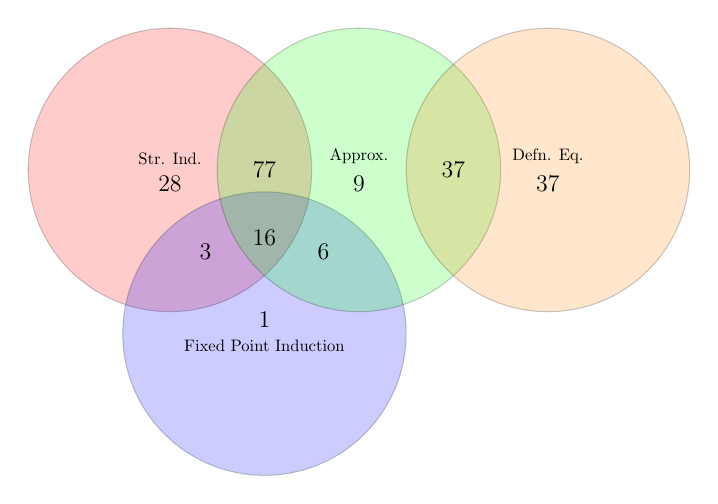
\begin{tikzpicture}[scale=0.6]
  \tikzset{venn circle/.style={draw,circle,minimum width=6cm,fill=#1,opacity=0.2}}

  \node [venn circle = red]    (S) at (0,0)                              {};
  \node [venn circle = blue]   (F) at (-60:4cm)                          {};
  \node [venn circle = green]  (A) at (0:4cm)                            {};
  \node [venn circle = orange] (P) at (0:8cm)                            {};
  \node [above]                    at (barycentric cs:S=1)               {Str. Ind.};
  \node [below]                    at (barycentric cs:S=1)               {\resS};
  \node [above]                    at (barycentric cs:F=1)               {\resF};
  \node [below]                    at (barycentric cs:F=1)               {Fixed Point Induction};
  \node [above]                    at (barycentric cs:A=1)               {Approx.};
  \node [below]                    at (barycentric cs:A=1)               {\resA};
  \node [above]                    at (barycentric cs:P=1)               {Defn. Eq.};
  \node [below]                    at (barycentric cs:P=1)               {\resP};
  \node [left]                     at (barycentric cs:S=1/2,F=1/2)       {\resSF};
  \node                            at (barycentric cs:S=1/2,A=1/2)       {\resSA};
  \node [right]                    at (barycentric cs:F=1/2,A=1/2)       {\resFA};
  \node [below]                    at (barycentric cs:S=1/3,F=1/3,A=1/3) {\resSFA};
  \node                            at (barycentric cs:A=1/2,P=1/2)       {\resPA};

\end{tikzpicture}

  \caption{Venn diagram of intersection between proved theorems for
    different techniques. The data is from the 214 proved theorems
    when using all provers.
    \label{fig:venn}
  }
\end{figure}

There are a number of observations to do from this figure. The
different parts of the diagram is studied in the rest of this section.


\subsection{Definitional Equality and the Approximation Lemma}
\label{sec:defeqandapprox}

Firstly, definitional equality only overlaps with the approximation
lemma. The reason for this is that this technique is only applied when
all arguments are abstract, as outlined in Section
\ref{sec:concreteconcerns}. Further, fixed point induction is only
used for recursive functions and properties about such functions
generally need induction. Approximation lemma is applicable when the
type of the equality is concrete, so that is the source of the overlap.

The properties provable with definitional equality and the
approximation lemma naturally comes from properties regarding only
functions from files \ts{Functions}, \ts{MonadEnv} and
\ts{MonadState}, where definitional equality alone proves the
properties where the type of the equality is not concrete. Two
unit test properties could for these reasons also only be proved with
definitional equality, like this one from \ts{Queues}:

\begin{code}
prop_34 :: a -> Prop a
prop_34 x = top (enqueue x empty) =:= x
\end{code}

\noindent
Indeed, this property is not applicable for proving with any other
technique. There were about 10 unit test properties provable with both
approximation lemma and definitional equality.

\paragraph{Only Approximation Lemma}
The 9 properties provable with only approximation lemma can be divided
in two parts. The first part consists of a property from \ts{Streams}:

\begin{code}
zero :: Stream Nat
zero = pure Zero

one :: Stream Nat
one = pure (Succ Zero)

prop_one :: Prop (Stream Nat)
prop_one = Succ <$> zero =:= one
\end{code}

\noindent
Here, \hs{pure} is the infinite stream constructed by repeating a
value, and \hs{<\$>} is map over streams. This could be proved with
fixed point induction, but it currently does not do any
inlining. Should \hs{zero} be inlined to \hs{pure Z} and similarly for
\hs{one}, the property is provable with fixed point induction as well.
Note that fixed point induction is instantiated when the theory is
generated, so it does not help that the theorem provers can deduce that $\hs{zero} =
\hs{pure Zero}$.

The other 8 properties only proved with approximation lemma come from
\ts{MonadState}. This monad is written without a newtype wrapper, and
in many different ways. The implementations of bind with a strict
\hs{uncurry} definition and the property of right return identity are
stated in this file as this:

\begin{code}
-- Strict in its second argument. The normal definition uses a irrefutable pattern.
uncurry f (a,b) = f a b

(>>=) :: State s a -> (a -> State s b) -> State s b
(m >>= f) s = uncurry f (m s)

return :: a -> State s a
return x s = (x,s)

prop_return_right_strict :: (s -> (a,s)) -> Prop (s -> (a,s))
prop_return_right_strict f = (f >>= return) =:= f
\end{code}

\noindent
The property will be expanded to \hs{(f >>= return) s =:= f s}.
Interestingly, proving this with the approximation lemma works as a
typing predicate: it will provide the information that \hs{f s} is
either bottom or \hs{(a,b)} for some \hs{a} and \hs{b}. This
information is not available for the untyped setting in definitional
equality and thus gets stuck.


\paragraph{Approximation Lemma and Fixed Point Induction}
The properties provable with only these two techniques all come from
\ts{Infinite}, and include properties about \hs{map}, \hs{repeat},
\hs{iterate} and similar constructions for Trees rather than
lists. Neither of these properties have concrete arguments to do
structural induction on.

\subsection{Structural Induction}
\label{sec:strindres}

The properties provable with only structural induction include
properties from \ts{Fix}, where ordinary functions are written in
terms of \hs{fix}, where fixed point induction ironically does not
work. In addition, many properties come are about natural numbers and
lists.

Some structural induction and approximation lemma theorems are
essentially doing proof by plain equality but with cases, from
\ts{Bool}. However, most of them come from properties about lists and
natural numbers, integers and the \hs{Maybe} monad.

\paragraph{Structural Induction and Fixed Point Induction}
The three properties provable with only these two techniques point
induction come from \ts{IWC}, \ts{Infinite} and \ts{Nat}
respectively. The first is a definition of proving the equivalence
between a mutually recursive definition of an even predicate over
natural numbers and a self-recursive definition in depth two. The
first is readily not provable with the approximation lemma as it
approximates the resulting \hs{Bool}, and a stronger induction
hypothesis is needed.

The second property is one of the functor laws for \hs{fmap} for trees:

\begin{code}
prop_fmap_comp :: (b -> c) -> (a -> b) -> Tree a -> Prop (Tree c)
prop_fmap_comp f g t = fmap (f . g) t =:= fmap f (fmap g t)
\end{code}

\noident
Interestingly, this property is provable with the approximation lemma,
but it takes more than 5 seconds: the E theorem prover produces a
proof in 18s.

The last property does not seem to be suitable for approximation:

\begin{code}
prop_max_assoc :: Nat -> Nat -> Nat -> Prop Nat
prop_max_assoc a b c = max (max a b) c =:= max a (max b c)
\end{code}

\paragraph{Using all inductive techniques}
The properties provable with all three techniques are associativity
proofs, symmetry of \hs{max} from \ts{Nat}, some properties about
lists from \ts{ZenoLists} and some lemmas from
\ts{ProductiveUseOfFailure}, including:

\begin{code}
prop_L7 :: a -> a -> [a] -> Nat -> Nat -> Nat -> Prop [a]
prop_L7 x y zs m n o = drop (S o) (drop n (drop (S m) (x:y:zs)))
                   =:= drop (S o) (drop n (drop m (x:zs)))
\end{code}

\subsection{Fixed Point Induction and Exponential Types}
There was only one property only provable with fixed point induction,
namely the property of associative addition for Brouwer ordinals from
\cite{dixonphd} in the test file \ts{Ordinals}. The relevant
definitions are these:

\begin{code}
data Ord = Zero | Suc Ord | Lim (Nat -> Ord)

(+) :: Ord -> Ord -> Ord
Zero  + b = b
Suc a + b = Suc (a + b)
Lim f + b = Lim (\n -> f n + b)

prop_assoc_plus :: Ord -> Ord -> Ord -> Prop Ord
prop_assoc_plus a b c = a + (b + c) =:= (a + b) + c
\end{code}

\noindent
The \hs{Ord} data type is exponential, and complete support for such
types were never implemented for structural induction and the
approximation lemma (see Section \ref{sec:futind}). With fixed point
induction, this support comes for free. For the proof of associativity
the fixed functions are the first addition in both sides, with this
induction hypothesis:

\newcommand{\Lim}{\fn{lim}}
\newcommand{\pw}{\fixw{+}}
\newcommand{\pb}{\fixb{+}}

\begin{equation*}
\faaa{a}{b}{c} a \pw (b + c) = (a \pw b) + c
\end{equation*}

\noindent
The interesting case is for the limit $\Lim(f)$ in the step part of
proof by fixed point induction. A proof that liberally uses
lambdas instead of explicit pointers is given below:

\begin{align*}
lhs = & \; \Lim (f) \pb \big(b + c\big)                       && \{\textrm{definition of $\pb$}\}\\
    = & \; \Lim (\lambda n . f(n) \pw \big(b + c\big))        && \{\textrm{induction hypothesis}\}\\
    = & \; \Lim (\lambda n . (f(n) \pw b) + c)                && \{\textrm{$\beta$-expansion}\}\\
    = & \; \Lim (\lambda n . (\lambda m . f(m) \pw b)(n) + c) && \{\textrm{definition of $+$}\}\\
    = & \; \big(\Lim (\lambda m . f(m) \pw b\big) + c         && \{\textrm{definition of $\pb$}\}\\
    = & \; \big(\Lim (f) \pb b\big) + c = \; rhs
\end{align*}

In hindsight, it is not so surprising that this property is provable
with fixed point induction, but its applicability on exponential data
types was actually not thought of during its implementation.

\section{Results for Different Theorem Provers}

In this section we present how well the different provers succeeded on
the big run of the test suite. As in the previous section, successes for
methods which handle all values are called Theorems, and for methods
that only work on finite and total values are called Finite Theorems.

To compare the provers and the different proof methods on this test
suite, the number of proved properties for each prover and proof
method is illustrated in Table \ref{tbl:proved}. The entries in the
row captioned Theorem shows how many theorems were proved out of the
total. The following four columns for definitional equality,
structural induction, approximation lemma and fixpoint induction tells
how many properties out of those could be proved with this method. The
following two columns are similar, though for finite theorems where the
only applicable method is structural induction.

\begin{table}[h]
\centering
%\documentclass{article}
%\usepackage{fullpage}
%\usepackage{courier}

%\usepackage{amssymb}
%\usepackage{longtable}
%
%\begin{document}
%
%\title{Results}
%\maketitle

%\section*{Total}
\begin{tabular}{>{\small}l || >{\small}r@{/}>{\small}l | >{\small}r@{/}>{\small}l | >{\small}r@{/}>{\small}l | >{\small}r@{/}>{\small}l | >{\small}r@{/}>{\small}l || >{\small}r@{/}>{\small}l | >{\small}r@{/}>{\small}l}
Prover & \multicolumn{2}{>{\small}l|}{Theorem} & \multicolumn{2}{>{\small}l|}{defn.eq.} & \multicolumn{2}{>{\small}l|}{induction} & \multicolumn{2}{>{\small}l|}{approx} & \multicolumn{2}{>{\small}l||}{fixpoint} & \multicolumn{2}{>{\small}l|}{Finite Thm.} & \multicolumn{2}{>{\small}l}{induction} \\
\hline
E           & 203&540 & 68&203 & 120&203 & 136&203 & 23&203 &  99&540 &  99&99\\
prover9     & 194&540 & 69&194 & 114&194 &  92&194 &  8&194 &  93&540 &  93&93\\
SPASS       & 198&540 & 65&198 & 122&198 & 111&198 & 21&198 &  94&540 &  94&94\\
Vampire     & 208&540 & 71&208 & 122&208 & 133&208 & 25&208 & 104&540 & 104&104\\
equinox     &  78&540 & 15&78  &  57&78  &  56&78  &  3&78  &  39&540 &  39&39\\
\hline
all provers & 214&540 & 74&214 & 124&214 & 145&214 & 26&214 & 111&540 & 111&111\\
\hline
\end{tabular}

%\end{document}

\caption{Number of proved properties per prover and proof method.
         Only the Theorem is counted for properties proved as both
         Theorems and Finite Theorems.
\label{tbl:proved}
}
\end{table}

\paragraph{Discussion}
In general, all provers tested in this experiment but equinox
performed almost equally well on this problem set. For those four in
the top the differences are small, but the most successful is
Vampire. It is closely followed by E, which performs slightly better on
the approximation lemma. One of the notable differences is that
prover9 performs worse proofs by the approximation lemma and fixed
point induction. The theorem provers has been considered as
black-boxes and examining these results in terms of how the theorem
provers operate is out of scope of this thesis.

\begin{comment}

A striking observation is that the approximation lemma is the most
successful of proving techniques for Theorems. As we saw in the
previous section, it intersects definitional equality on 37
properties, and 8 of its uniquely proved properties could be proved
with definitional equality if it had more typing information, and the
last one if fixed point induction did more inlining. However, after
definitional equality, it is also the easiest to formulate and
implement.

Structural induction could become even stronger if the combinatorial
explosion when generating induction hypotheses could be
restricted. Currently, it creates all smaller trees than the induction
conclusion, but another alternative is to use all sub trees.

Definitional equality is only applicable for properties with only
abstract arguments. There are some notable files in the test suite
with these, \ts{Functions}, \ts{MonadEnv} and \ts{MonadState}, and
most successes come from there. Should the translation be changed so
that it also applicable on concrete arguments, it would also be able
to prove properties from for example \ts{Bool}, and intersect
structural induction that currently proves these techniques.


\section{Results per File}

To compare the different kinds of properties from the files of the
test suite the results per file can be viewed in Table
\ref{tbl:allstats}.

\begin{table}[h]
%\centering
%\documentclass{article}
%\usepackage{fullpage}
%\usepackage{courier}
%\usepackage{amssymb}
%\usepackage{longtable}
%
%\begin{document}
%
%\title{Results}
%\maketitle
%
%\section*{ home dan remote run 4442 evpsx statistics.data}
\begin{tabular}{>{\footnotesize}l || >{\footnotesize}c | >{\footnotesize}c | >{\footnotesize}c | >{\footnotesize}c | >{\footnotesize}c || >{\footnotesize}c | >{\footnotesize}c}
File                       & Thm & defn.eq. & ind & approx & fixpoint & Fin.Thm. & ind \\
\hline
$\ts{Bool                    }$   & 15/23 & 2/15 & 13/15 & 15/15 &  & 8/23 & 8/8\\
$\ts{Expr                    }$   & 4/8 &  & 4/4 & 3/4 & 1/4 &  & \\
$\ts{Fix                     }$   & 7/7 &  & 7/7 & 1/7 &  &  & \\
$\ts{Functions               }$   & 15/19 & 15/15 &  &  &  & 4/19 & 4/4\\
$\ts{IWC                     }$   & 2/7 &  & 2/2 & 1/2 & 2/2 &  & \\
$\ts{Infinite                }$   & 11/15 &  & 5/11 & 10/11 & 9/11 &  & \\
$\ts{InsertionSort           }$   &  &  &  &  &  & 1/12 & 1/1\\
$\ts{Integers                }$   & 7/14 &  & 7/7 & 6/7 &  & 6/14 & 6/6\\
$\ts{MergeSort               }$   &  &  &  &  &  &  & \\
$\ts{MonadEnv                }$   & 18/18 & 18/18 &  &  &  &  & \\
$\ts{MonadMaybe              }$   & 10/10 & 2/10 & 8/10 & 10/10 &  &  & \\
$\ts{MonadState              }$   & 33/48 & 25/33 &  & 31/33 &  &  & \\
$\ts{Nat                     }$   & 11/33 &  & 11/11 & 6/11 & 3/11 & 15/33 & 15/15\\
$\ts{Nat2ndArg               }$   & 4/18 &  & 4/4 & 4/4 & 1/4 & 5/18 & 5/5\\
$\ts{NatAcc                  }$   & 2/18 &  & 2/2 & 2/2 &  & 1/18 & 1/1\\
$\ts{NatDouble               }$   & 2/18 &  & 2/2 & 2/2 &  & 8/18 & 8/8\\
$\ts{NatDoubleSlow           }$   & 2/18 &  & 2/2 & 2/2 &  & 8/18 & 8/8\\
$\ts{NatStrict               }$   & 4/18 &  & 4/4 & 3/4 &  & 6/18 & 6/6\\
$\ts{NatSwap                 }$   & 4/18 &  & 4/4 & 3/4 &  & 1/18 & 1/1\\
$\ts{Ordinals                }$   & 2/6 &  & 1/2 & 1/2 & 1/2 &  & \\
$\ts{PatternMatching         }$   & 9/15 & 4/9 & 5/9 & 7/9 &  & 6/15 & 6/6\\
$\ts{ProductiveUseOfFailure  }$   & 6/85 &  & 6/6 & 6/6 & 6/6 & 21/85 & 21/21\\
$\ts{Queues                  }$   & 14/23 & 7/14 & 7/14 & 9/14 &  & 2/23 & 2/2\\
$\ts{Reverse                 }$   & 9/17 & 1/9 & 8/9 & 9/9 & 1/9 & 1/17 & 1/1\\
$\ts{Sequences               }$   &  &  &  &  &  &  & \\
$\ts{Streams                 }$   & 1/3 &  &  & 1/1 &  &  & \\
$\ts{Tricky                  }$   &  &  &  &  &  & 4/8 & 4/4\\
$\ts{ZenoLists               }$   & 22/54 &  & 22/22 & 13/22 & 2/22 & 14/54 & 14/14\\
\hline
Total                      & 214/540 & 74/214 & 124/214 & 145/214 & 26/214 & 111/540 & 111/111\\
\end{tabular}
%\end{document}

\caption{Number of proved properties per file and proof method, using
  all provers. An empty cell means nothing proved.
\label{tbl:allstats}
}
\end{table}

\paragraph{Discussion}

These results shreds some light over the success of approximation
lemma: it is applicable for non recursive structures. That enables it
to prove properties from \ts{Bool} and \ts{MonadMaybe}, as well as on
the tuple result in \ts{MonadState}. On the other hand, fixed point
induction is only for recursive functions. It performs well on the
tests suited for it, notably the Infinite file, but also surprisingly
on the Theorems from \ts{ProductiveUseOfFailure} which are only
contains properties about lists and natural numbers.

The two files \ts{Nat} and \ts{ZenoLists} are taken from the Zeno test
suite \citep{zeno}. Zeno accomplishes to prove all but two properties,
and the situation is a bit different here. If the theorems and finite
theorems are summed, the result is 26/33 for \ts{Nat} and 36/54 for
\ts{ZenoLists}. The explanation is simple, our tool neither use nor
discover lemmas, whereas Zeno can. A similar result can be found in
the test suite file \ts{ProductiveUseOfFailure} from the paper with
the same name \citep{productiveuse}. The tests from that paper
includes the lemmas discovered by their tool, and most of the theorems
we can prove are those lemmas. Lemmas are crucial in many files,
examples are \ts{InsertionSort} and \ts{Reverse}. It is also needed to
prove more sophisticated properties not widely included in this test
suite.

\end{comment}


\section{Proving Time}

Most invocations to the theorem provers are solved in a few
milliseconds, and few can take up to 500 ms. SPASS had the largest
success time of all invocation: about 1500ms, but that was the only
success over one second. The cumulative amount of success times can be
viewed in Figure \ref{fig:provingtime}. Each method can give rise to
several different ways of proving a property, an example is fixed
point induction on different functions, and each of these can consist
of one or many invocations to a theorem prover, an example is the base
and the different step cases in a proof by structural induction.  All
invocations from a technique with a given setting that ended in
success are counted in the figure.


\begin{figure}[h]
\centering
\begin{tikzpicture}
\begin{axis}[xlabel={time (ms)},ylabel=quantity,
             enlargelimits=false,ymax=3000,ymin=0,
             width=10cm,
             xmin=0,xmax=500]
\addplot [draw=black] table[x=time,y=qty]  {resultdata/theoremTimes.data} ;
\end{axis}
\end{tikzpicture}
\caption{Cumulative amount of successes over time, using all provers
  and methods. Only successes from a method resulting in a theorem are counted.
\label{fig:provingtime}
}
\end{figure}

\paragraph{Discussion}
The figure conveys that more than the majority of invocations for
successes take less than 50ms, and after 300ms almost no new successes
are encountered. However, as noticed in Section \ref{sec:strindres},
there are also examples where much longer invocation times are
needed. A way of guiding the theorem provers in the search space of
proofs is discussed in Section \ref{sec:minpredicate}.

\begin{comment}
The theorem provers are well suited for these kinds of problems, with
some variance already discussed. This motivates using automated
theorem provers to prove properties about Haskell programs. For the
specific setup, 5 seconds were used as timeout, but one second should
be sufficient, possibly less.
\end{comment}

